\documentclass[9pt]{beamer}

% apparence
\usetheme{Singapore}
\usecolortheme{orchid}
\setbeamercolor{title}{
    use=structure,fg=white,bg=structure.fg!75!black
}
\useinnertheme[shadow]{rounded}

% numéro des slides
\addtobeamertemplate{navigation symbols}{}{
    \usebeamerfont{footline}
    \usebeamercolor[fg]{footline}
    \hspace{1em}
    \raisebox{2pt}{
        \insertframenumber/\inserttotalframenumber
    }
}

% réduire l'espace sous les titres de slides
\addtobeamertemplate{frametitle}{}{\vspace*{-5mm}}

% packages
\usepackage{mathtools}
\usepackage{graphicx, multirow}
\usepackage{algorithm, algpseudocode}
\usepackage[dvipsnames]{xcolor}

% titre du beamer
\title{A Clustered Approach to Adaptive Kriging Particle Filter for Magnetic Field-Aided Navigation}

\author{
    Bastien HUBERT\inst{1, 2},
    Karim DAHIA\inst{1},\\
    Nicolas MERLINGE\inst{1},
    Audrey GIREMUS\inst{2}
}

\institute{
    \inst{1} ONERA, DTIS, IGNC\quad
    \inst{2} Université de Bordeaux, CNRS, IMS
}

\date{}

\titlegraphic{
    \vspace{-\baselineskip}
    
\includegraphics[width=10cm]{../../Images/Logo ONERA IMS.pdf}
}

% début du beamer
\begin{document}

\begin{frame}

\begin{center}
    \includegraphics[width=2.5cm]{../../Images/Logo EUSIPCO 2025.png}
    \hspace{1cm}
    \raisebox{5pt}{\includegraphics[width=2cm]{../../Images/Logo IEEE.png}}
    \vspace{-\baselineskip}
\end{center}

\titlepage

\end{frame}

\logo{
    \includegraphics[width=1cm]{../../Images/Logo EUSIPCO 2025.png}
    \hspace{2mm}
    \raisebox{1pt}{\includegraphics[width=1cm]{../../Images/Logo IEEE.png}}
    \hspace{4.5cm}
    
\includegraphics[width=5cm]{../../Images/Logo ONERA IMS.pdf}
}

\section{Introduction}

\begin{frame}{Context: autonomous navigation for UAVs}

\begin{block}{Inertial navigation for unmanned aerial vehicles (UAVs)}
    \begin{itemize}
    \item Integrates measurements from the accelerometers and gyrometers of an inertial measurement unit
    \item Autonomous and reliable on short missions
    \item But imperfect measures (biases, scale factors, noises, ...)
    \item[$\Rightarrow$] Drifts over time
    \end{itemize}
\end{block}

\begin{block}{Data fusion}
    \begin{itemize}
    \item Using data from other sensors helps reduce the drift
    \item GNSS as an ideal counterpart to inertial data, but not always available
    \item[$\Rightarrow$] Physical field-aided navigation instead
    \item Measures from exteroceptive onboard sensors
    \item Comparison between the measured data and an embedded map
    \end{itemize}
\end{block}

\end{frame}

\begin{frame}{Magnetic field-aided navigation}

\begin{block}{Earth's magnetic anomaly field}
    \begin{itemize}
    \item Measurement of the local field by a magnetometer
    \item Decomposition and extraction of the magnetic anomaly:\\
    \hfill$\displaystyle\mathcal{B}_{total}=\mathcal{B}_{core}+\boxed{\mathcal{B}_{crust}}+\mathcal{B}_{UAV}+\mathcal{B}_{external}$\hfill(1)
    \item Comparison with a georeferenced embedded map
    \end{itemize}
\end{block}

\begin{columns}[onlytextwidth]
\begin{column}{0.55\textwidth}

\begin{block}{Challenges}
    \begin{itemize}
    \item High initial state uncertainty
    \item Non-linear and non-injective environment model
    \item Noisy and poorly-known environment
    \end{itemize}
\end{block}

\end{column}
\begin{column}{0.42\textwidth}

\begin{center}
    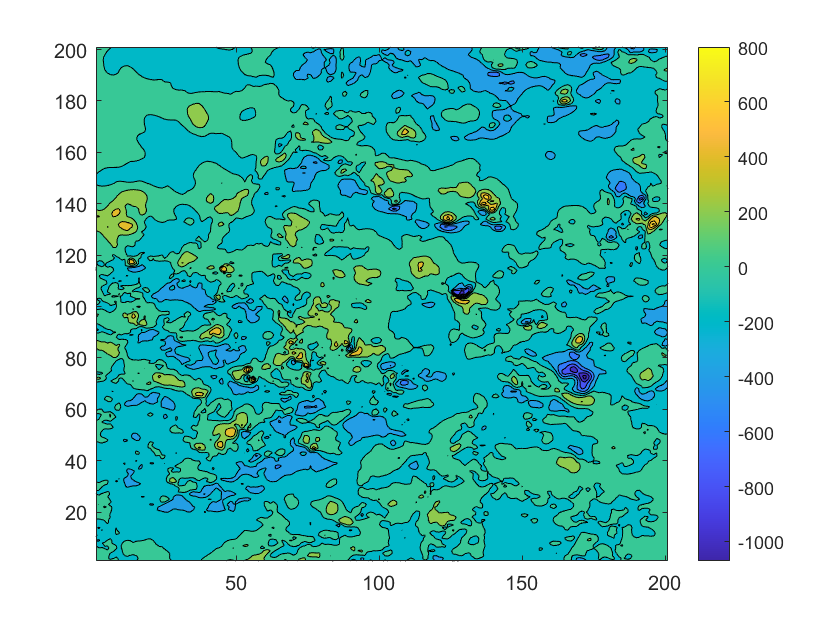
\includegraphics[width=\textwidth]{../../Images/Carte magnétométrique EUSIPCO 2025.png}
\end{center}

\end{column}
\end{columns}

\end{frame}

\section{Problem statement}

\begin{frame}{Bayesian estimation}

\begin{block}{Discrete state-space representation}
    \begin{itemize}
    \item\hfill$\displaystyle\setlength\arraycolsep{1pt}\left\{\begin{matrix*}[l]
    x_k&\sim&\mathcal{N}(&\mathcal{F}_k(x_{k-1}),&Q_k&)&\quad\text{recursive dynamical process}\\
    z_k&\sim&\mathcal{N}(&\mathcal{H}_k(x_k),&R_k&)&\quad\text{measurement equation}
    \end{matrix*}\right.$\hfill(2)
    \end{itemize}
\end{block}

\begin{block}{Bayesian filtering}
    \begin{itemize}
    \item Goal: compute $p(x_k|z_{1:k})$ the posterior probability density function (PDF)
    \item State estimation:\\
    \hfill$\displaystyle\hat{x}_k\triangleq\mathbb{E}(x_k|z_{1:k})=\int{x_k\:p(x_k|z_{1:k})\:dx_k}$\hfill(3)
    \item Error covariance matrix:\\
    \hfill$\displaystyle P_k\triangleq\mathbb{V}(\hat{x}_k)=\int{(x_k-\hat{x}_k)(x_k-\hat{x}_k)^Tp(x_k|z_{1:k})\:dx_k}$\hfill(4)
    \end{itemize}
\end{block}

\end{frame}

\begin{frame}{Bayesian estimation}

\begin{block}{Optimal Bayesian filter}
    \begin{itemize}
    \item Recursive process in two steps:
    \begin{itemize}
    \item Prediction step with Chapman-Kolmogorov's equation:\\
    \hfill $\displaystyle p(x_k|z_{1:k-1})=\underbrace{\int{p(x_k|x_{k-1})\:p(x_{k-1}|z_{1:k-1})\:dx_{k-1}}}_{\text{no analytical solution}}$\hfill(5)
    \item Correction step with Bayes' formula:\\
    \hfill $\displaystyle p(x_k|z_{1:k})=\frac{p(z_k|x_k)\:p(x_k|z_{1:k-1})}{\int{p(z_k|x_k)\:p(x_k|z_{1:k-1})\:dx_k}}$\hfill(6)
    \end{itemize}
    \end{itemize}
\end{block}

\begin{columns}[onlytextwidth]
\begin{column}{0.55\textwidth}

\begin{block}{Kalman filter}
    \begin{itemize}
    \item Optimal analytical estimation under strong assumptions: linear equations and Gaussian noises
    \item Poorly handles ambiguities and multi-modality
    \item[$\Rightarrow$] Stochastic methods are superior in these cases
    \end{itemize}
\end{block}

\end{column}
\begin{column}{0.4\textwidth}

\begin{center}
    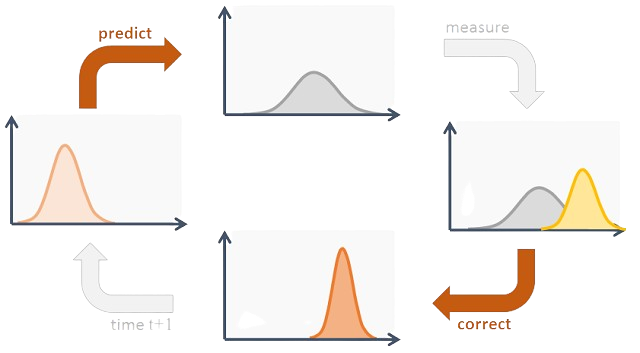
\includegraphics[width=\textwidth]{../../Images/Étapes du filtre de Kalman avec images.png}
\end{center}

\end{column}
\end{columns}

\end{frame}

\begin{frame}{Particle filtering}

\begin{block}{Standard particle filter}
    \begin{itemize}
    \item Importance sampling method
    \item \scalebox{0.96}{Asymptotically optimal under weak assumptions: $\mathcal{F}_k$, $\mathcal{H}_k$, $Q_k$ and $R_k$ known}
    \item Posterior PDF approximation using a mixture of Dirac distributions:\\
    \hfill$\displaystyle p(x_k|z_{1:k})\approx\sum_{i=1}^Nw_k^i\delta_{x_k^i}(x_k)$\hfill(7)
    \item Prediction step with proposal density $q$:\vspace{0.5\baselineskip}\\
    \hfill$\displaystyle x_k^i\sim q(x_k|x_{k-1}^i,z_k)=p(x_k|x_{k-1}^i)$\hfill(8)
    \item Correction step:\\
    \hfill$\displaystyle w_k^i\propto w_{k-1}^i\frac{p(z_k|x_k^i)\:p(x_k^i|x_{k-1}^i)}{q(x_k^i|x_{k-1}^i,z_k)}=w_{k-1}^ip(z_k|x_k^i)$\hfill(9)
    \end{itemize}
\end{block}

\end{frame}

\begin{frame}{Auxiliary particle filter (APF)}

\begin{block}{Auxiliary particle filter}
    \begin{itemize}
    \item Particle degeneracy during the correction step
    \item[$\Rightarrow$] Introduction of auxiliary particles to assess the likelihood of future particles
    \item New pre-propagation and pre-correction steps:\\
    \hfill$\displaystyle\setlength\arraycolsep{1pt}\left\{\begin{aligned}
    \mu_k^i\sim p(x_k|x_{k-1}^i)\\
    \lambda_k^i\propto w_{k-1}^ip(z_k|\mu_k^i)
    \end{aligned}\right.$\hfill$\begin{aligned}(10)\\(11)\end{aligned}$
    \item Degeneracy mitigated by resampling auxiliary particles and propagating their parents accordingly
    \item Updated correction:\\
    \hfill$\displaystyle w_k^j\propto\frac{p(z_k|x_k^j)}{p(z_k|\mu_k^{i^j})}$\hfill(12)
    \end{itemize}
\end{block}

\end{frame}

\section{Adaptive Kriging Particle Filter}

\begin{frame}{Gaussian process regression}

\begin{block}{Navigation in poorly-known environment}
    \begin{itemize}
    \item Poorly-known environment $\rightarrow$ Bayesian correction is impossible
    \item[$\Rightarrow$] Kriging grants an analytical expression of the measurement function and noise conditional to some training data
    \end{itemize}
\end{block}

\begin{columns}[onlytextwidth]
\begin{column}{0.3\textwidth}

\begin{center}
    \hspace*{-10mm}
    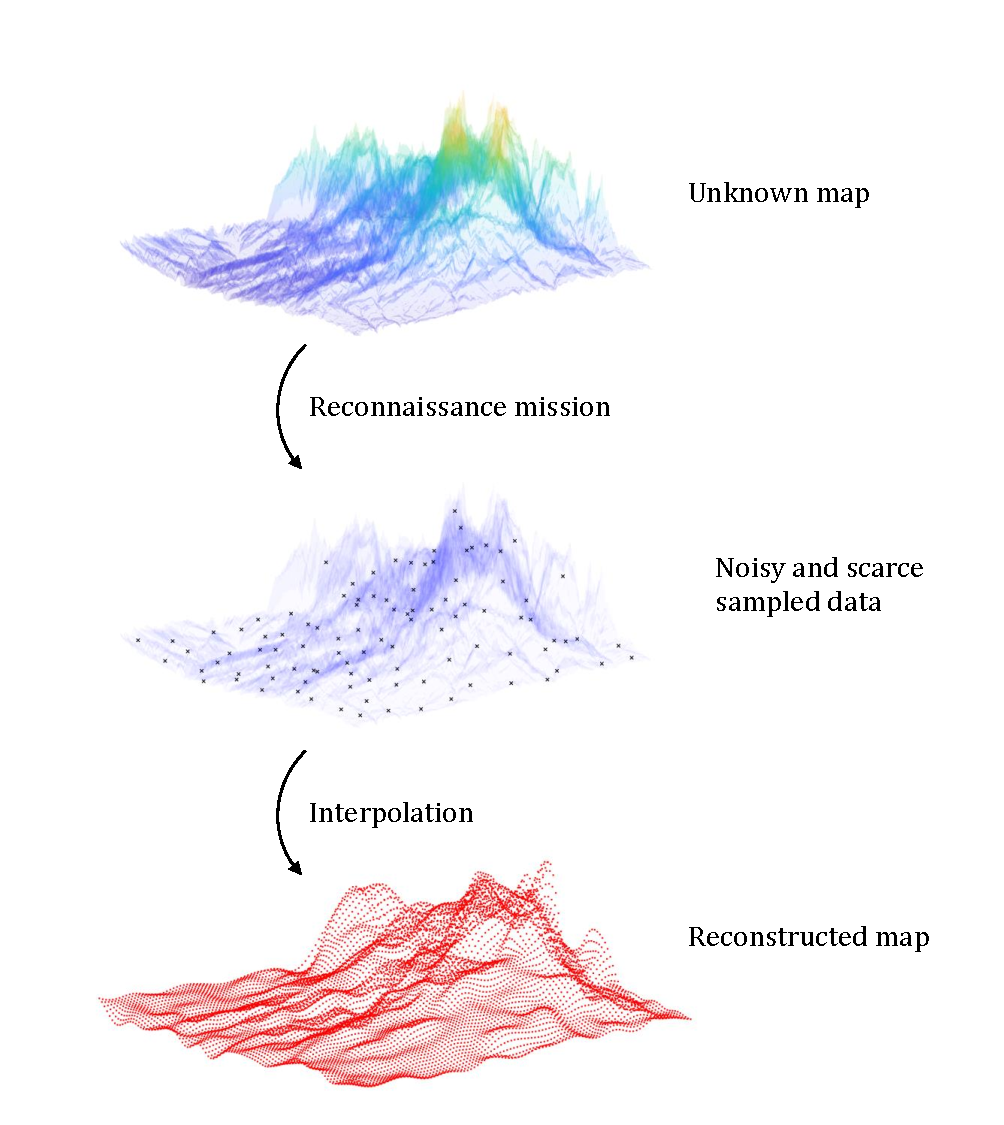
\includegraphics[width=\dimexpr\textwidth+8mm\relax]{../../Images/Étapes du krigeage.pdf}
\end{center}

\end{column}
\begin{column}{0.7\textwidth}

\begin{block}{Gaussian process regression}
    \begin{itemize}
    \item Particles and training data:\\
    \hfill\hspace{-1cm}$\displaystyle\setlength\arraycolsep{1pt}\left\{\begin{matrix*}[l]
    &z&\sim&\mathcal{GP}(&0,&\mathcal{K}(x,x)+R&)\\
    \forall i\in[\![1,\tilde{N}]\!],&\tilde{z}^i&\sim&\mathcal{GP}(&0,&\mathcal{K}(\tilde{x}^i,\tilde{x}^i)+\tilde{R}&)
    \end{matrix*}\right.$\hfill(13)\vspace{2mm}
    \item Conditional probability distribution:\\
    \hfill\hspace{-1cm}$\displaystyle\setlength\arraycolsep{1pt}\left\{\begin{aligned}
    z^*(x,\tilde{X},\tilde{Z})=&\mathcal{K}(x,\tilde{X})\left(\mathcal{K}(\tilde{X},\tilde{X})+\tilde{R}\otimes I_{\tilde{N}}\right)^{-1}\tilde{Z}\\
    R^*(x,\tilde{X})=&\mathcal{K}(x,\tilde{X})\left(\mathcal{K}(\tilde{X},\tilde{X})+\tilde{R}\otimes I_{\tilde{N}}\right)^{-1}\mathcal{K}(\tilde{X},x)\hspace{-10mm}
    \end{aligned}\right.$\hfill(14)
    \end{itemize}
\end{block}

\end{column}
\end{columns}

\end{frame}

\begin{frame}{Clustered adaptive kriging (CAK)}

\begin{columns}[onlytextwidth]
\begin{column}{0.35\textwidth}

\begin{center}
    \hspace{-10mm}
    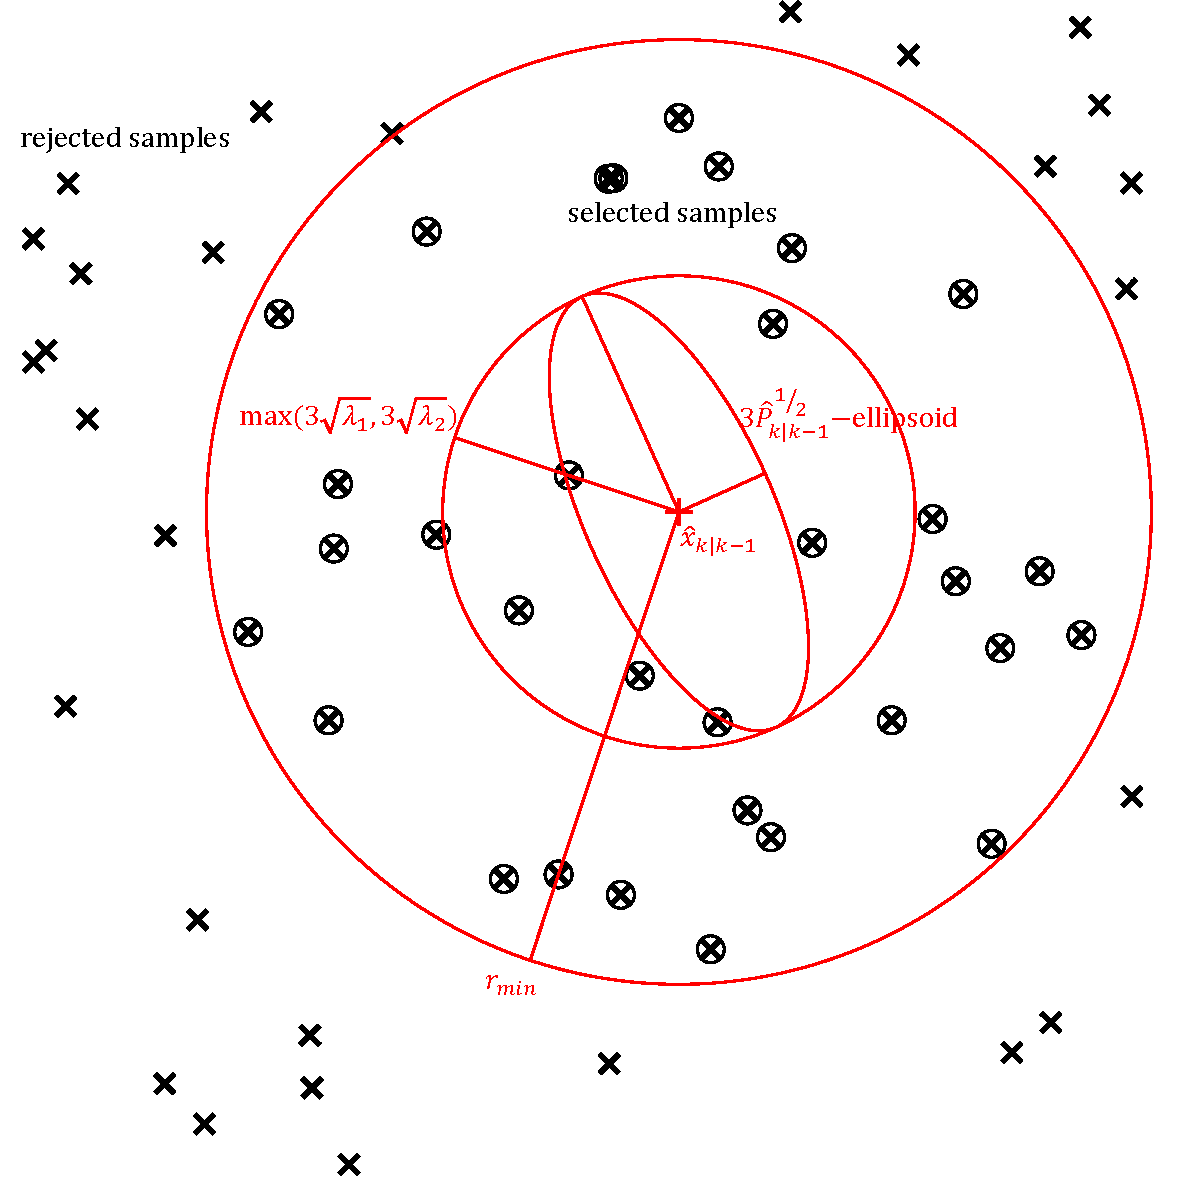
\includegraphics[width=\textwidth]{../../Images/Fenêtrage du krigeage adaptatif.pdf}
\end{center}

\end{column}
\begin{column}{0.65\textwidth}

\begin{block}{Training data selection}
    \begin{itemize}
    \item Non-stationarity of the correction field
    \item Need to select relevant training data
    \item Adaptive selection set:\\
    \hfill$S_k\triangleq\mathcal{B}\left(\hat{x}_{k|k-1},\alpha\times\underset{\lambda\in\text{sp}(P_{k|k-1})}{\text{max}}\left(3\sqrt{\lambda}\right)\right)$\hfill(15)
    \end{itemize}
\end{block}

\end{column}
\end{columns}

\begin{columns}[onlytextwidth]
\begin{column}{0.65\textwidth}

\begin{block}{Clustering the particles}
    \begin{itemize}
    \item In case of multimodality, $S_k$ can become large
    \item Skews hyperparameter estimation and increases PF computational load
    \item[$\Rightarrow$] Clustering to solve both issues
    \item Kriging around each clustered estimated state
    \end{itemize}
\end{block}

\end{column}
\begin{column}{0.3\textwidth}

\begin{center}
    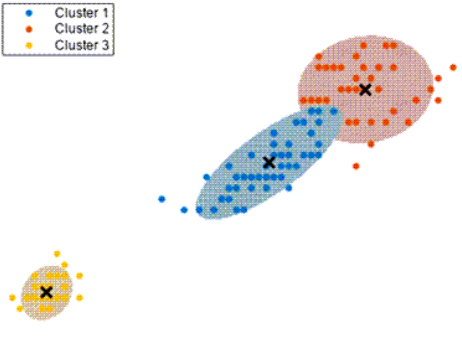
\includegraphics[width=\textwidth]{../../Images/Exemple de clustering.png}
\end{center}

\end{column}
\end{columns}

\end{frame}

\begin{frame}{CAK-APF pseudo-code}

\begin{block}{Algorithm overview}
\begin{algorithmic}
    \State{$\forall i\in[\![1,N]\!]$, draw $\mu_k^i$ from $p(\cdot|x_{k-1}^i)$}\Comment{Pre-propagation}
    \State{\textcolor{BrickRed}{Determine the clusters $\{\mathcal{C}_k^l,l\in[\![1,c_k]\!]\}$}}\textcolor{BrickRed}{\Comment{Clustering}}
    \For{$l\in[\![1,c_k]\!]$}
    \State{\textcolor{BrickRed}{Compute $S_k^{\mathcal{C}_k^l}$ with clustered (15)}}\textcolor{BrickRed}{\Comment{Adaptive selection}}
    \For{$\mu_k^i\in\mathcal{C}_k^l$}
    \State{\textcolor{BrickRed}{Compute $z^*_k$ from clustered adaptive (14)}}\textcolor{BrickRed}{\Comment{Kriging}}
    \State{Compute $\lambda_k^i$ from (11)}\Comment{Pre-correction}
    \EndFor
    \EndFor
    \State{Normalise $\{\lambda_k^i,i\in[\![1,N]\!]\}$}\Comment{Normalisation}
    \State{$\{i^j,j\in[\![1,N]\!]\}=\text{Resample}(\{\lambda_k^i,i\in[\![1,N]\!]\})$}
    \For{$j\in[\![1,N]\!]$}
    \State{Draw $x_k^j$ from $p(\cdot|x_{k-1}^{i^j})$}\Comment{Propagation}
    \State{\textcolor{BrickRed}{Associate $x_k^j$ to the cluster containing $\mu_k^{i^j}$}}
    \State{\textcolor{BrickRed}{Compute $z^*_k$ from clustered adaptive (14)}}\textcolor{BrickRed}{\Comment{Kriging}}
    \State{Compute $w_k^i$ from (12)}\Comment{Correction}
    \EndFor
    \State{Normalise $\{w_k^j,j\in[\![1,N]\!]\}$}\Comment{Normalisation}
    \end{algorithmic}
\end{block}

\end{frame}

\section{Numerical results}

\begin{frame}{Simulation}

\begin{block}{Simulation parameters}
    \begin{itemize}
    \item Uniform rectilinear motion
    \item 100 Monte Carlo trials per filter
    \end{itemize}
    \begin{center}
    \begin{tabular}{rl}\hline
    Parameters&Value\\\hline
    Number of particles&5000\\
    Kernel function&Gaussian kernel\\
    Resampling algorithm&Kitagawa\\
    Clustering algorithm&Mean-shift\\
    Number of iterations&$600$\\
    Map surface&$200\text{km}\times200\text{km}$\\
    Initial error covariance&$\text{diag}([3000\text{m},3000\text{m},3\text{m.s}^{-1},3\text{m.s}^{-1}])^2$\\
    Evolution covariance&$\text{diag}([40\text{m},40\text{m},0.4\text{m.s}^{-1},0.4\text{m.s}^{-1}])^2$\\
    Measurement covariance&$80^2\text{ nT}^2$\\
    Number of training data&$80^2$\\
    Training measurement covariance&$80^2\text{ nT}^2$\\\hline
    \end{tabular}
    \end{center}
\end{block}

\end{frame}

\begin{frame}{Example of an estimated trajectory}

\begin{columns}
\begin{column}{0.45\textwidth}

\begin{center}
    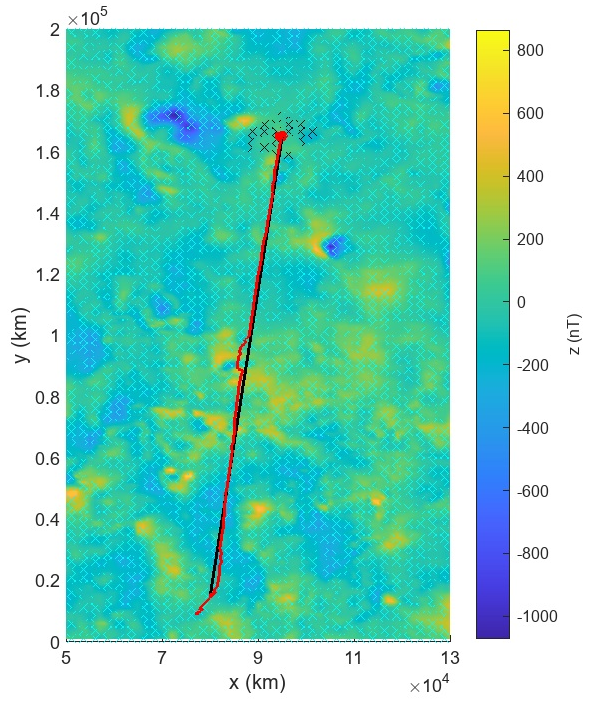
\includegraphics[width=\textwidth]{../../Images/Trajectoire EUSIPCO 2025 fin.pdf}
\end{center}

\end{column}
\begin{column}{0.55\textwidth}

\begin{center}
    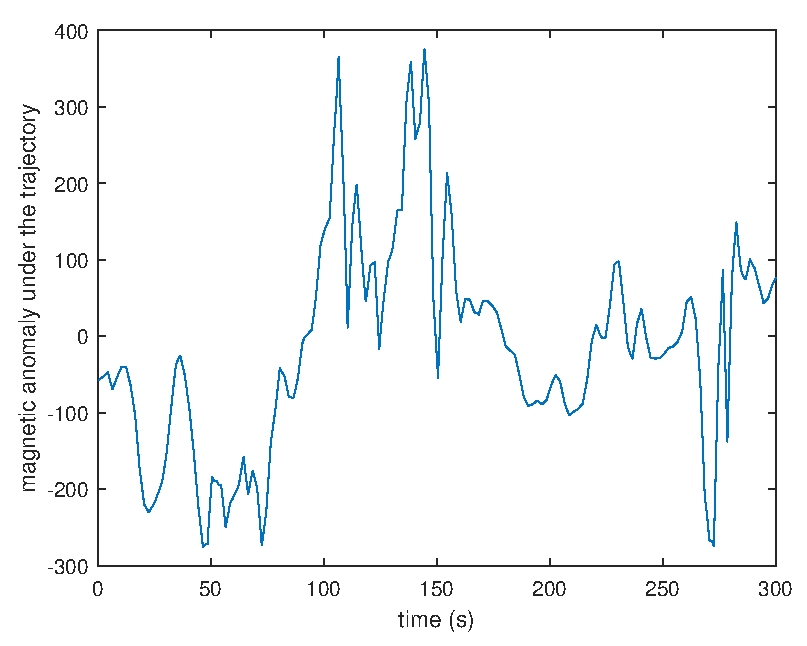
\includegraphics[width=\textwidth]{../../Images/Anomalie magnétique EUSIPCO 2025.pdf}
\end{center}

\end{column}
\end{columns}

\end{frame}

\begin{frame}{Ablation study of CAK-APF}

\begin{columns}[onlytextwidth]
\begin{column}{0.55\textwidth}

\begin{center}
    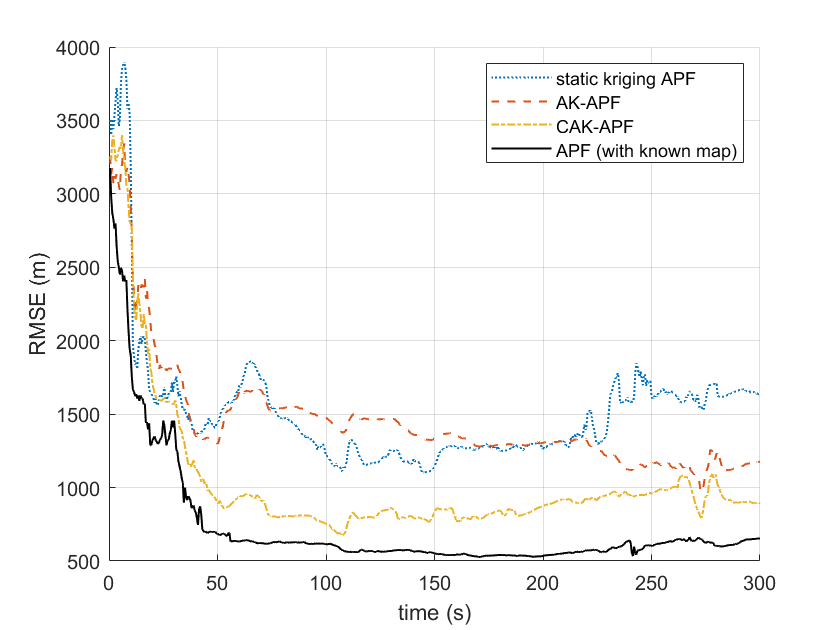
\includegraphics[width=\textwidth,height=0.7\textheight]{../../Images/RMSE EUSIPCO 2025.png}
\end{center}

\end{column}
\begin{column}{0.45\textwidth}

\begin{center}
    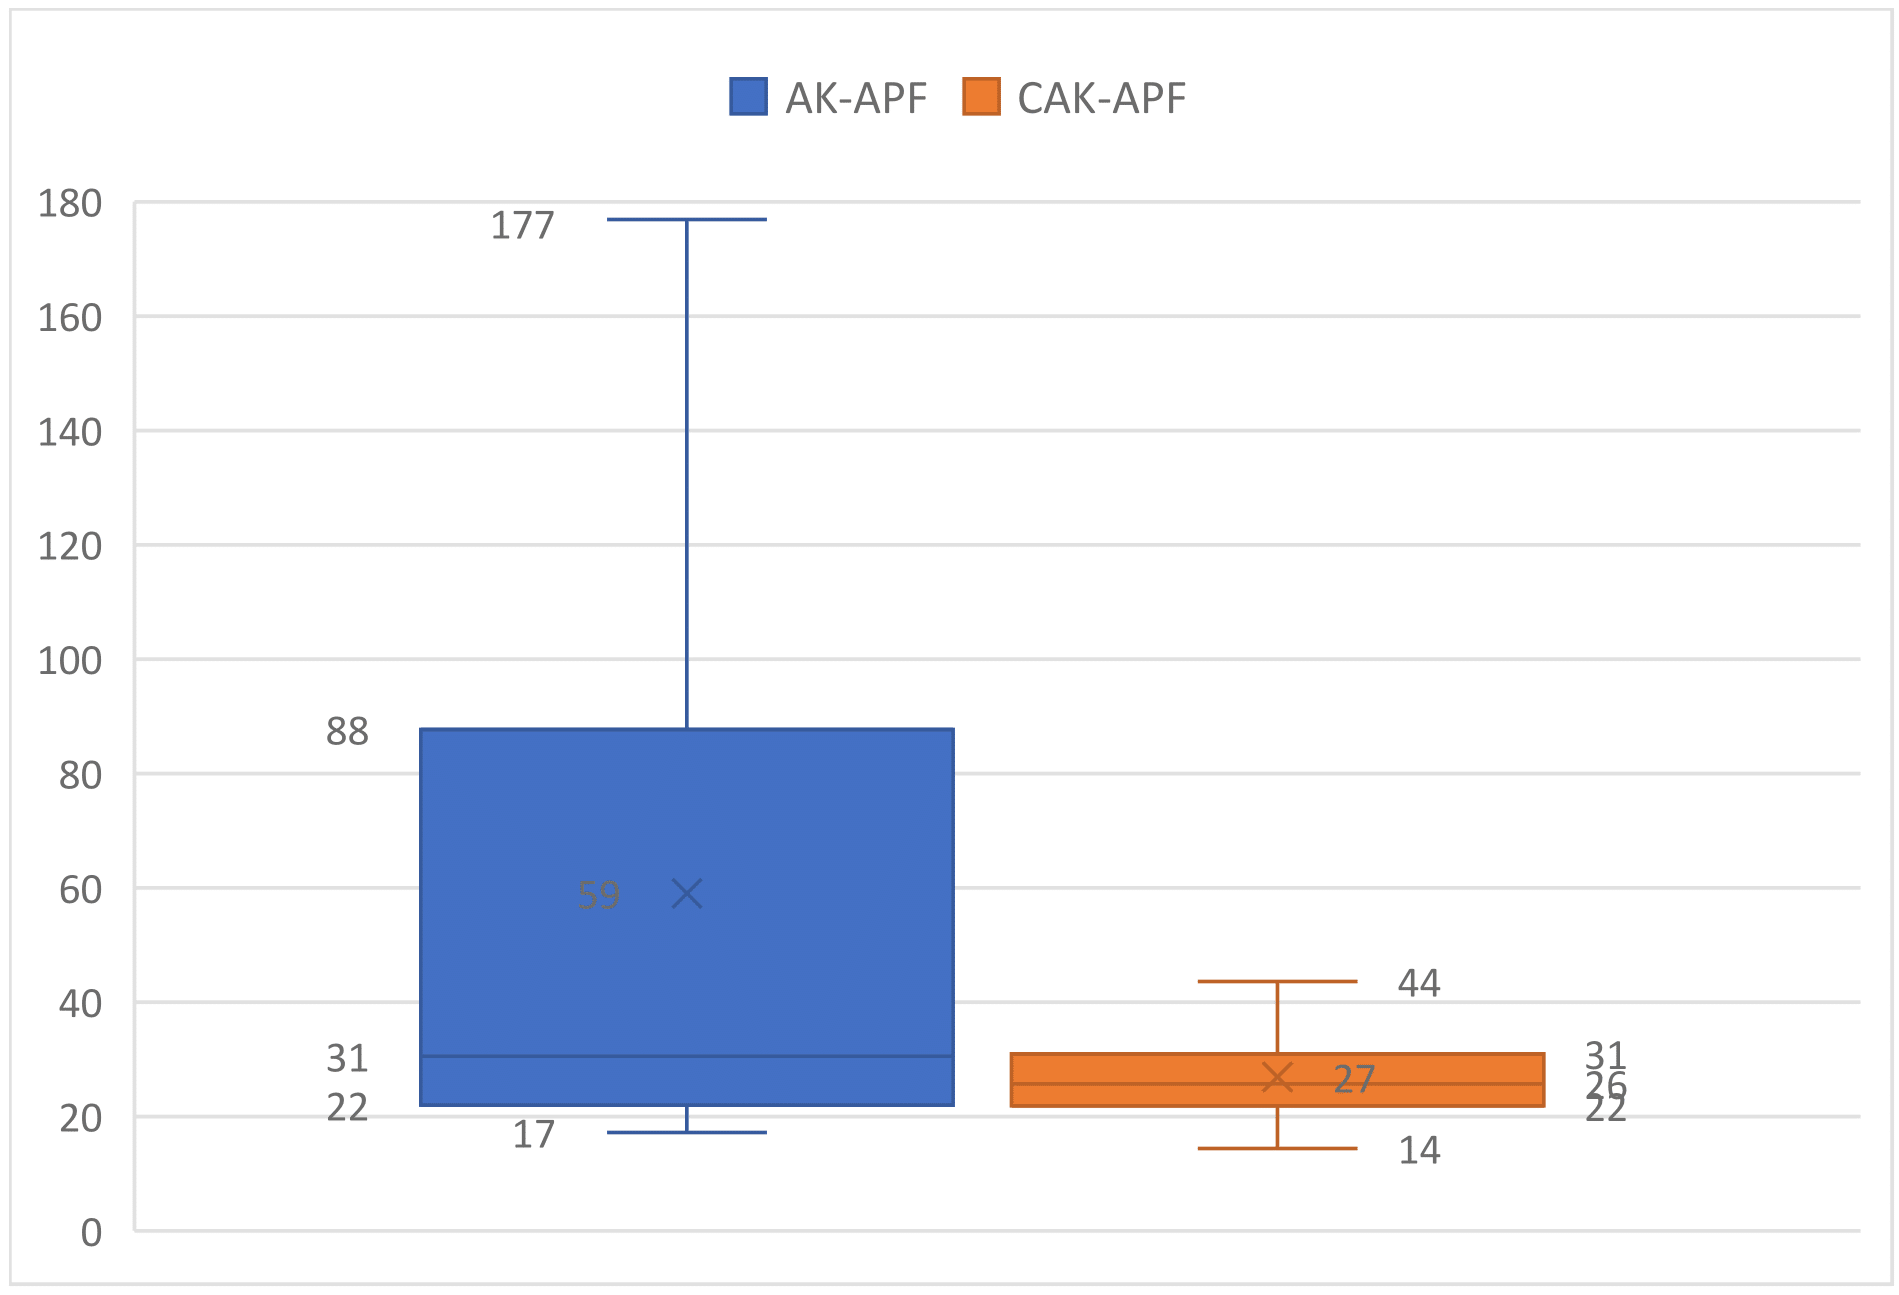
\includegraphics[width=\textwidth,height=0.6\textheight]{../../Images/Histogramme du nombre de données krigées EUSIPCO 2025.png}
\end{center}

\end{column}
\end{columns}

\end{frame}

\begin{frame}{Conclusion and future work}

\begin{block}{Our work}
    \begin{itemize}
    \item Local adaptive reconstruction of the Earth's magnetic anomaly field in a poorly-known environment
    \item Reduced computational load by introducing a clustering step in the adaptive selection
    \item Ablation study of CAK-APF to assess the impact of each module to the overall performance
    \end{itemize}
\end{block}

\begin{block}{Perspectives}
    \begin{itemize}
    \item Exploration of new data selection methods
    \item Formal estimation of the interpolation error induced by the selection
    \item Simultaneous localisation and mapping (SLAM) formalism to eliminate the need of prior training data
    \end{itemize}
\end{block}

\end{frame}

\end{document}
